\documentclass[12pt,a4paper]{ctexart}

\usepackage{geometry}
\geometry{left=2.6cm,right=2.6cm,top=2.5cm,bottom=2.4cm}
\usepackage{amsmath,amssymb,amsthm}
\usepackage{booktabs}
\usepackage{graphicx}
\usepackage{float}
\usepackage{caption}
\usepackage{array}
\usepackage{multirow}
\usepackage{enumitem}
\usepackage{xcolor}
\usepackage{fancyhdr}
\usepackage[hidelinks]{hyperref}

\captionsetup{font=small,labelsep=quad}
\setlength{\parskip}{0.35em}
\linespread{1.45}
\renewcommand{\arraystretch}{1.15}

\newtheorem{theorem}{定理}
\newtheorem{lemma}{引理}
\newtheorem{definition}{定义}
\newtheorem{remark}{注}

\pagestyle{fancy}
\fancyhf{}
\fancyhead[L]{\small 图上随机游走与个性化重启的马尔可夫链模型}
\fancyhead[R]{\small 吴桐}
\fancyfoot[C]{\small \thepage}
\setlength{\headheight}{14pt}
\renewcommand{\headrulewidth}{0.4pt}

\title{\vspace{-1.2cm}\textbf{图上随机游走与个性化重启的马尔可夫链模型}\\[4pt]
\large 以 MovieLens 评分网络为例}
\author{}
\date{}

\begin{document}

% ============================ 封面 ============================
\begin{titlepage}
\centering
\vspace*{2.2cm}
{\zihao{2}\bfseries 图上随机游走与个性化重启的马尔可夫链模型\par}
\vspace{0.5cm}
{\zihao{4} 以 MovieLens 评分网络为例\par}
\vspace{3.2cm}
{\zihao{4}
\centering
学\hspace{1em}院：理学院\\[10pt]
专业班级：数学与应用数学2024-02班\\[18pt]
授课教师：艾晓辉\\[18pt]
姓\hspace{1em}名：吴桐\\[18pt]
学\hspace{1em}号：2024213023\par}
\vfill
{\zihao{5}\today\par}
\end{titlepage}

% ============================ 摘要 ============================
\begin{center}
{\zihao{4}\bfseries 摘\quad 要}
\end{center}

本文把 MovieLens 100K 的评分关系建成加权图，并在图上定义带重启项的随机游走，作为四个问题共用的对象。状态取评分数最多的 200 部电影，边权取用户评分向量的余弦相似度，每个节点仅保留相似度最高的 20 个邻居，由此得到 $200$ 个状态、$3028$ 条边的稀疏转移矩阵 $P$。转移再以
\[
P_{\alpha}=\alpha P+(1-\alpha)\mathbf{1}v^{\top}
\]
的概率回到先验 $v$，得到 $P_{\alpha}$，其中 $v$ 为个性化先验。其每个元素均不小于 $(1-\alpha)v_j>0$，故链不可约且非周期；Perron--Frobenius 定理保证平稳分布唯一，且任意初始分布均收敛于该分布，此 $\pi$ 即个性化 PageRank 得分。数值上 $\alpha$ 取 $0.6$，幂迭代 40 次后 $L_1$ 残差为 $9.19\times10^{-13}$，与直接解方程组的解相差 $1.13\times10^{-12}$，谱隙 $0.449$。数据按时间戳切为四片，逐片重估 $\pi_t$；第 4 片的预测取 $\hat p_4=f_3P_{\alpha^*}$，即由第 3 片的实际分布 $f_3$ 推进一期而非直接使用平稳分布，得 KL $0.0451$、Spearman $0.781$，二者在四组方法中均为最优（Top-10 命中率低于纯热门，$0.30$ 对 $0.60$）。用户级个性化预测的 NDCG@10 为 $0.211$、覆盖率 $0.635$，纯热门为 $0.365$。关闭重启项时 $P_{\alpha}$ 退化为 $P$，更换种子结果不变，个性化消失，这从反面说明了该充项的必要性。

\vspace{0.6em}
\noindent\textbf{关键词：}\ 马尔可夫链；随机游走；个性化重启；平稳分布；PageRank；MovieLens

\newpage
\tableofcontents
\newpage

% ============================ 1 问题陈述 ============================
\section{问题陈述}

\subsection{背景与意义}

马尔可夫链刻画的是“下一步只依赖当前状态”的随机演化，与历史无关\cite{norris}。围绕这一定义，问题的重点落在状态空间的选取、转移矩阵的计算与极限行为三处。本文的四步也由此展开：问题 1 求状态空间的种类，问题 2 计算转移概率矩阵，问题 3 讨论极限分布与平稳分布的关系，问题 4 由历史数据推断未来分布。
本文选择图上随机游走作为载体。图上的随机游走天然是马尔可夫链，转移只依赖当前节点，边权由用户评分给出。此外，带重启的随机游走在工程上即个性化 PageRank\cite{page,haveliwala}，问题 3 的平稳分布因此具有明确含义，问题 4 亦可用带时间戳的数据加以检验。

需要说明的是，问题 4 的“状况分布”既可指全体物品的热度分布，也可指单个用户自身分布。本文对两者分别处理：全局层面以一步马尔可夫推进检验分布演化，用户层面以个性化重启构造推荐并作离线评估。

\subsection{数据与任务}

数据取自 GroupLens 公开的 MovieLens 100K 数据集\cite{movielens}：$100{,}000$ 条评分，$943$ 位用户，$1682$ 部电影，评分取值 $1$--$5$，时间跨度 1997-09-20 至 1998-04-22。本文的任务是：

\begin{enumerate}[label=(\arabic*),leftmargin=2.2em]
\item 明确状态空间的种类，构造马尔可夫链；
\item 计算该链的转移概率矩阵；
\item 求出极限分布，并判断它是否为平稳分布；
\item 利用历史数据刻画状态分布及其演化，预测未来分布，并与基线比较。
\end{enumerate}

% ============================ 2 问题分析 ============================
\section{问题分析}

\subsection{推荐问题转化为链上概率转移}

推荐系统的常见做法是“找相似”\cite{jeh,fouss}：与用户已评分物品相似的物品更可能被选中。随机游走把相似性转化为可执行的跳转——若两部电影被同一批用户评分且评分向量接近，则在二者之间连一条带权边，粒子由当前节点按边权比例选择下一步。相似度据此成为转移概率，多步游走相当于沿相似关系作幂次传播，推荐排序即平稳分布的降序。

\subsection{前置知识}

问题 1 需要状态空间的分类语言：状态可数与否、链可约与否、有无周期、常返或瞬态。问题 2 需构造非负且行和为 $1$ 的随机矩阵，并说明稀疏性与计算复杂度。问题 3 依赖非负矩阵的 Perron--Frobenius 理论\cite{pf}与幂迭代的收敛速率估计\cite{levin}，难点在于区分“极限分布”与“平稳分布”，并证明本模型下二者重合。问题 4 需随时间重估参数，以条件分布推进一期，并以 KL 散度、Top-10 命中率、Spearman 秩相关评价预测质量。

\subsection{技术路线}

计算流程分三阶段：预处理阶段将评分整理为用户--物品矩阵 $R$，计算物品间余弦相似度，经 Top-$K$ 截断与行归一化得到 $P$；计算阶段实现 $P_{\alpha}$ 并以幂迭代求 $\pi$，同时以直接解线性方程组交叉验证，再按时间四分位切为四片逐片重估；评估阶段完成全局分布预测与用户级个性化预测，各设三个基线。

% ============================ 3 问题求解 ============================
\section{问题求解}

\subsection{问题 1：状态空间的种类与链的构造}

\subsubsection{状态空间}

以全体电影为潜在状态空间规模过大，且长尾部分缺少共同评分者，边无从定义。因此本文先作一次显式筛选：按评分数降序取前 $N=200$ 部电影，构成状态集
\[
S=\{1,2,\dots,200\},\qquad |S|=200 .
\]
本文的筛选规则为\textbf{按评分数排序取前 200}，评分数区间 $151$--$583$，不按类型与时间筛选；这 200 部电影覆盖 $47{,}825$ 条评分，占全数据的 $47.8\%$。状态空间属可数、有限类型，链为离散时间马尔可夫链。

\subsubsection{边的构造}

设 $U_i$ 为给电影 $i$ 评过分的用户集合，$r_{ui}$ 为用户 $u$ 对电影 $i$ 的评分。定义两物品的余弦相似度
\begin{equation}
s_{ij}=\frac{\sum_{u\in U_i\cap U_j} r_{ui}\,r_{uj}}
{\sqrt{\sum_{u\in U_i} r_{ui}^{2}}\ \sqrt{\sum_{u\in U_j} r_{uj}^{2}}}\in[0,1],
\label{eq:cos}
\end{equation}
分子仅在共同评分者上累加，分母取各自全部评分的模长。该定义存在已知偏向：共同评分者较少但评分一致时，相似度仍可较高。为控制噪声与稀疏性，每个节点仅保留相似度最高的 $K=20$ 个邻居，并作对称化
\begin{equation}
w_{ij}=\max\{s_{ij},s_{ji}\}\,\mathbf{1}\{\,j\in N_K(i)\ \text{或}\ i\in N_K(j)\,\},
\label{eq:w}
\end{equation}
其中 $N_K(i)$ 为 $i$ 的 Top-$K$ 邻居集。对称化的原因在于相似关系未必彼此成立；若仅保留单向边，链的有向结构与图的无向直觉不一致。

得到的图有 $200$ 个节点、$3028$ 条无向边，平均度 $30.28$，最大度 $113$，加权平均度 $16.26$，边权范围 $0.2714$--$0.8845$，密度 $0.1522$。全网只有 $1$ 个连通分量，无孤立节点，说明在全体数据上这张图是连通的。

\subsubsection{链的分类性质}

无向连通图上的简单随机游走不可约，周期性则等价于图是否为二部图。本图存在由共同评分关系构成的三角形，非二部，故链在全体数据上既不可约又非周期，$P$ 本身已有唯一平稳分布。这一点须如实说明：\textbf{就全量数据而言，“可约性”并非由重启项解决}。

可约性实际出现在逐时间片重估。表 \ref{tab:slices} 显示第 1、2 片均只有 $196$ 个节点连成主分量，另有 $4$ 个节点在该片内无任何共同评分者而完全悬挂。此时 $P^{(t)}$ 可约，平稳分布不唯一，极限分布取决于初始分布所落入的闭 communicating class。重启项的必要性正在此处，后文将回到这一点。

\begin{table}[H]
\centering
\caption{四个时间片的基本统计（按评分时间戳四分位切分）}
\label{tab:slices}
\small
\begin{tabular}{cccccccc}
\toprule
片号 & 起止日期 & 评分数 & 用户数 & 连通分量 & 主分量 & 悬挂节点 & $\pi_t$ 熵 \\
\midrule
1 & 1997-09-20 $\sim$ 1997-11-13 & 11957 & 270 & 5 & 196 & 4 & 5.214 \\
2 & 1997-11-13 $\sim$ 1997-12-18 & 11956 & 271 & 5 & 196 & 4 & 5.214 \\
3 & 1997-12-18 $\sim$ 1998-02-21 & 11957 & 342 & 1 & 200 & 0 & 5.222 \\
4 & 1998-02-21 $\sim$ 1998-04-22 & 11955 & 359 & 1 & 200 & 0 & 5.235 \\
\bottomrule
\end{tabular}
\end{table}

从常返性看，有限状态不可约链的所有状态均正常返，不存在瞬态；而逐片可约链中，悬挂节点一旦进入便无法离开，成为吸收态，属“吸收型”退化。该对照直接反映链结构的差异。

\subsection{问题 2：转移概率矩阵的构造}

\subsubsection{行归一化与悬挂处理}

由边权矩阵 $W=(w_{ij})$ 定义转移矩阵
\begin{equation}
P_{ij}=\frac{w_{ij}}{\sum_{k\in S}w_{ik}},\qquad i,j\in S .
\label{eq:P}
\end{equation}
行和为 $1$，$P$ 为随机矩阵。度数为 $0$ 的悬挂节点行归一化无定义，本文以重启分布 $v$ 填充该行，即无路可走时按先验重新开始，以避免概率质量流失。

\subsubsection{重启项}

设 $v=(v_1,\dots,v_{200})^{\top}$ 为严格正的重启分布（$\sum_j v_j=1$），定义
\begin{equation}
P_{\alpha}=\alpha P+(1-\alpha)\mathbf{1}v^{\top},\qquad \alpha\in[0,1).
\label{eq:Palpha}
\end{equation}
其中 $\mathbf{1}$ 为全 $1$ 列向量。展开成分量形式：
\begin{equation}
P_{\alpha}(i,j)=\alpha P_{ij}+(1-\alpha)v_j .
\label{eq:Palpha-ij}
\end{equation}
其直观含义为：粒子以概率 $\alpha$ 沿图走一步，以概率 $1-\alpha$ 被拉回至按 $v$ 抽样得到的节点。$v$ 的选取决定个性化方向——取全局热门度 $v^{\mathrm{pop}}_j\propto$ 评分数，得到全局 PageRank；取单用户历史，得到该用户的个性化 PageRank。

单用户先验仅在少数物品上具有权重，若直接使用会使部分 $P_{\alpha}(i,j)$ 严格为 $0$。为此在实现中对用户先验作混合
\begin{equation}
v_u=(1-\varepsilon)\,\tilde v_u+\varepsilon\, v^{\mathrm{pop}},\qquad \varepsilon=0.15,
\label{eq:vu}
\end{equation}
其中 $\tilde v_u$ 为用户历史物品上的归一化权重，$v^{\mathrm{pop}}$ 为热门度，$\varepsilon=0.15$。这样 $v_u$ 严格为正，定理 \ref{thm:unique} 的条件得以成立。

\subsubsection{稀疏性与复杂度}

$200$ 个状态的理论最大边数 $19{,}900$，实际最大边数 $3028$ 条，即 $84.8\%$ 的位置为空。以稀疏矩阵存储时，单次矩阵--向量乘法复杂度为 $O(|E|)=O(3028)$，稠密形式为 $O(N^2)=O(40{,}000)$；这正是幂迭代单次迭代处于毫秒量级的原因。图的布局与 $\pi$ 的分布见图 \ref{fig:network}。

\begin{figure}[H]
\centering
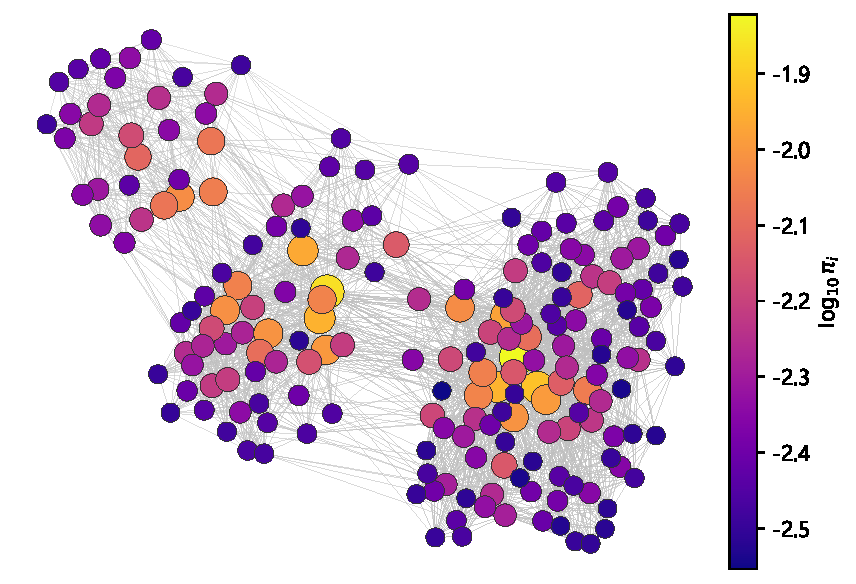
\includegraphics[width=0.72\textwidth]{fig/network.pdf}
\caption{物品共现图（200 节点、3028 边）。节点亮度与大小为 $\log_{10}\pi_i$，边缘粗细为相似度权重 $w_{ij}$。可见高分电影集中在图的几个稠密核，长尾节点沿边缘分布。}
\label{fig:network}
\end{figure}

\subsection{问题 3：极限分布与平稳性}

\subsubsection{唯一平稳性的证明}

\begin{theorem}\label{thm:unique}
设 $v_j>0$ 对一切 $j$ 成立，$\alpha\in[0,1)$，则 $P_{\alpha}$ 不可约、非周期，存在唯一的平稳分布 $\pi$（$\pi^{\top}=\pi^{\top}P_{\alpha}$，$\pi^{\top}\mathbf{1}=1$），且对任意初始分布 $\mu$ 有 $\|\mu^{\top}P_{\alpha}^{k}-\pi^{\top}\|_1\to 0$。
\end{theorem}

\begin{proof}
由式 \eqref{eq:Palpha-ij}，$P_{\alpha}(i,j)\ge(1-\alpha)v_j>0$ 对一切 $i,j$ 成立，故 $P_{\alpha}$ 是严格正矩阵，特别地 $P_{\alpha}^{m}$ 对所有 $m\ge1$ 都严格正。因此链不可约（任意两状态互通），且 $P_{\alpha}(i,i)>0$ 给出非周期。正矩阵的本原性由 Perron--Frobenius 定理保证：谱半径 $1$ 是单重特征值，对应唯一（归一化后）的左特征向量 $\pi$，其余特征值模严格小于 $1$。于是任意初始分布在该特征向量方向上的投影不变，其余分量按 $|\lambda_2|^{k}$ 衰减，极限存在且唯一。
\end{proof}

需要注意，该结论对 $P$ 本身一般\textbf{不成立}：$P$ 可能有多个闭类，平稳分布构成单纯形，极限依赖初始分布。定理 \ref{thm:unique} 的唯一性恰来自 $(1-\alpha)v_j$ 这一项。

\subsubsection{数值求解与双路验证}

幂迭代格式为
\begin{equation}
\pi_{k+1}^{\top}=\alpha\,\pi_k^{\top}P+(1-\alpha)\,v^{\top},\qquad
\pi_0^{\top}=v^{\top},
\label{eq:power}
\end{equation}
停止准则取 $\|\pi_{k+1}-\pi_k\|_1<10^{-12}$。等价的线性方程组形式为
\begin{equation}
(I-\alpha P^{\top})\,\pi=(1-\alpha)\,v,\qquad \pi^{\top}\mathbf{1}=1 .
\label{eq:linear}
\end{equation}
把式 \eqref{eq:linear} 的最后一行替换为归一化约束后直接求解，得到 $\pi^{\mathrm{dir}}$。两条路径的差异是检验“理论与代码一致性”的硬指标：

\begin{itemize}[leftmargin=1.6em]
\item $\alpha=0.6$ 时幂迭代 $40$ 次收敛，末残差 $9.19\times10^{-13}$；
\item 幂迭代解与直接解之间的 $L_1$ 距离 $1.13\times10^{-12}$；
\item 直接解代回平稳方程 \eqref{eq:power} 的残差 $7.25\times10^{-16}$（机器精度量级）；
\item 谱半径 $\lambda_1=1.000000$，次大特征值模 $|\lambda_2|=0.5511$，谱隙 $1-|\lambda_2|=0.4489$。
\end{itemize}

谱隙同时给出迭代步数的估计：误差每步约乘以 $\alpha|\lambda_2(P)|$。$\alpha=0.6$ 时收缩因子为 $0.5511$，$0.5511^{40}\approx4.4\times10^{-11}$，与实际 40 次迭代使误差由 $10^{-1}$ 降至 $10^{-12}$ 相吻合。残差曲线见图 \ref{fig:conv}，迭代数与谱隙随 $\alpha$ 的变化见图 \ref{fig:scan}。

\begin{figure}[H]
\centering
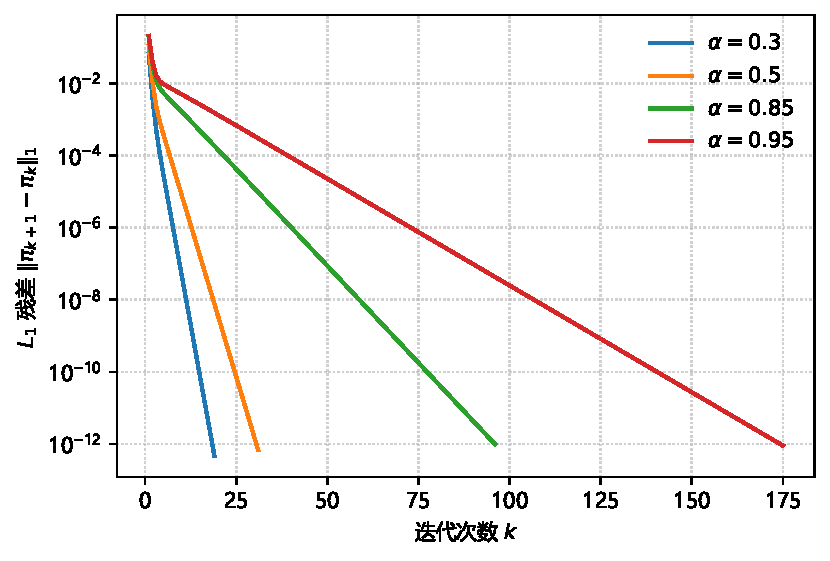
\includegraphics[width=0.60\textwidth]{fig/convergence.pdf}
\caption{不同 $\alpha$ 下的 $L_1$ 残差衰减（对数坐标）。$\alpha$ 越大，衰减越慢。}
\label{fig:conv}
\end{figure}

\begin{figure}[H]
\centering
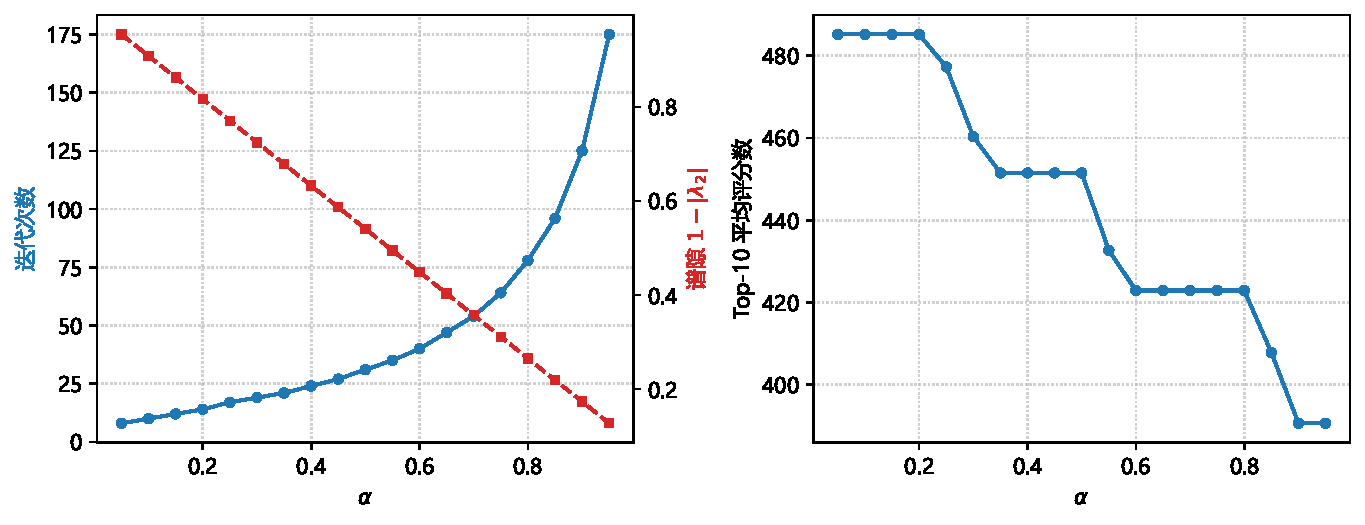
\includegraphics[width=0.94\textwidth]{fig/alpha_scan.pdf}
\caption{$\alpha$ 与迭代数（左轴）、谱隙（右轴）及 Top-10 平均评分数的关系。}
\label{fig:scan}
\end{figure}

$\alpha$ 由 $0.05$ 增至 $0.95$，迭代数由 $8$ 增至 $175$，谱隙由 $0.9541$ 降至 $0.1274$，二者近乎单调对应。可见 $\alpha$ 并非可任意设定的调参技巧，而是直接控制混合时间的量：$\alpha$ 越大，粒子越难被拉回，链越接近原图上的自由游走，混合越慢。

\subsubsection{极限分布是否就是平稳分布}

在本模型中：

\begin{enumerate}[label=(\arabic*),leftmargin=2.2em]
\item 由定理 \ref{thm:unique}，$P_{\alpha}$ 不可约非周期，故\textbf{极限分布存在}，且\textbf{等于}唯一平稳分布 $\pi$；
\item 但 $\pi$ 是 $P_{\alpha}$ 的平稳分布，\textbf{不是}原矩阵 $P$ 的平稳分布。二者只在 $\alpha\to1$ 时重合；
\item 当 $\alpha=1$ 时 $P_{\alpha}=P$，式 \eqref{eq:Palpha} 的个性化项消失，$P_{\alpha}$ 与 $v$ 完全无关。数值上，以用户先验与均匀先验分别迭代，两条轨迹的 $L_1$ 距离为 $0$，说明“换种子不换结果”，个性化失效。
\end{enumerate}

上述三者说明，重启后的平稳分布不等于原 $P$ 的平稳分布。数值上亦可看出差异：$\alpha=0.6$ 的 $\pi$ 熵为 $5.2137$，$\alpha=1$ 时为 $5.1577$，分布形状已然不同；$\pi$ 的集中程度随 $\alpha$ 变化（表 \ref{tab:alpha}）。

\begin{table}[H]
\centering
\caption{$\alpha$ 对收敛与分布形态的影响（全局先验 $v^{\mathrm{pop}}$）}
\label{tab:alpha}
\small
\begin{tabular}{cccccc}
\toprule
$\alpha$ & 迭代数 & $|\lambda_2|$ & 谱隙 & $\pi$ 熵 & Top-10 平均评分数 \\
\midrule
0.05 & 8   & 0.0459 & 0.9541 & 5.2423 & 485.2 \\
0.30 & 19  & 0.2756 & 0.7244 & 5.2310 & 460.3 \\
0.60 & 40  & 0.5511 & 0.4489 & 5.2137 & 422.9 \\
0.85 & 96  & 0.7807 & 0.2193 & 5.1954 & 407.8 \\
0.95 & 175 & 0.8726 & 0.1274 & 5.1826 & 390.6 \\
\bottomrule
\end{tabular}
\end{table}

表 \ref{tab:alpha} 最后一列值得单独说明：$\alpha$ 较小时 $\pi$ 接近热门度本身，Top-10 平均评分数为 $485.2$；$\alpha=0.95$ 时降至 $390.6$，排序由“绝对热门”转向“结构中心但未必最热”的物品。原型网页中“$\alpha$ 大偏冷门、$\alpha$ 小偏大众”的结论，依据即此列数据。

再考虑单种子情形：以评分数最多的《Star Wars (1977)》为唯一种子，$\alpha$ 由 $0.3$ 增至 $0.95$，种子自身概率质量由 $0.599$ 降至 $0.057$，$\pi$ 的熵由 $2.676$ 升至 $5.091$（表 \ref{tab:pers}）。可见 $\alpha$ 在此即“个性化强度”：较小时结果贴近种子，较大时被全网结构稀释。

\begin{table}[H]
\centering
\caption{单种子个性化下的 $\alpha$ 效应（种子为《Star Wars (1977)》）}
\label{tab:pers}
\small
\begin{tabular}{ccccc}
\toprule
$\alpha$ & 迭代数 & $\pi$ 熵 & 种子自身质量 & Top-10 平均评分数 \\
\midrule
0.30 & 20  & 2.676 & 0.599 & 442.0 \\
0.50 & 32  & 3.516 & 0.433 & 439.7 \\
0.70 & 57  & 4.278 & 0.267 & 439.7 \\
0.85 & 101 & 4.794 & 0.142 & 439.7 \\
0.95 & 182 & 5.091 & 0.057 & 432.5 \\
\bottomrule
\end{tabular}
\end{table}

$P_{\alpha}$ 的局部热图见图 \ref{fig:heat}；图 \ref{fig:longtail} 以双对数轴比较 $\pi$ 与纯热门度的长尾形状：$\pi$ 的头部质量为 $0.1149$，略高于热门度的 $0.1017$，尾部则更为平缓。可见重启链在保留头部的同时抬高中部节点，即“兼顾热门与结构相近”。

\begin{figure}[H]
\centering
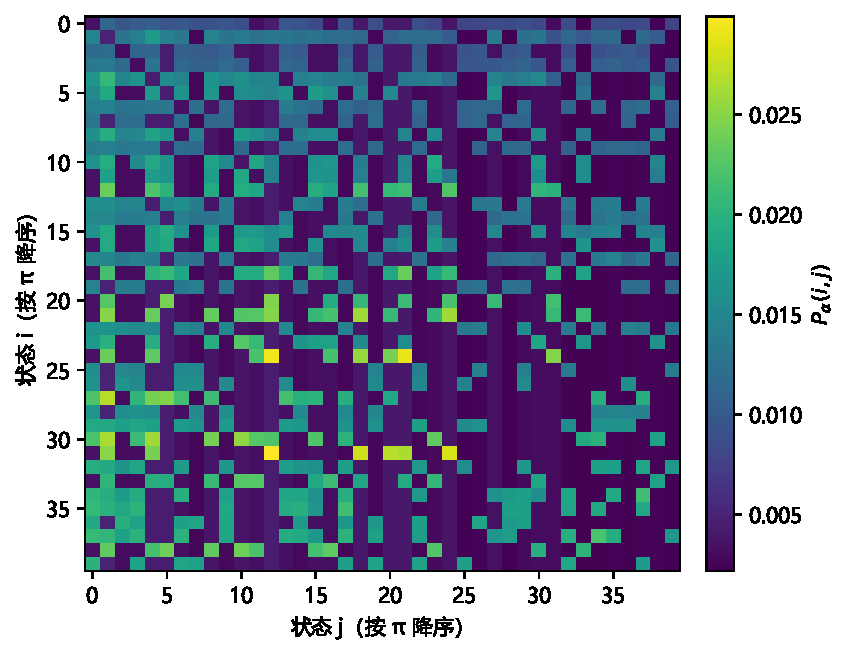
\includegraphics[width=0.56\textwidth]{fig/heatmap.pdf}
\caption{$P_{\alpha}$ 在 $\pi$ 最大的 40 个状态上的局部热图（$\alpha=0.6$）。对角与稠密块对应强相似邻居，整体底噪由重启项贡献。}
\label{fig:heat}
\end{figure}

\begin{figure}[H]
\centering
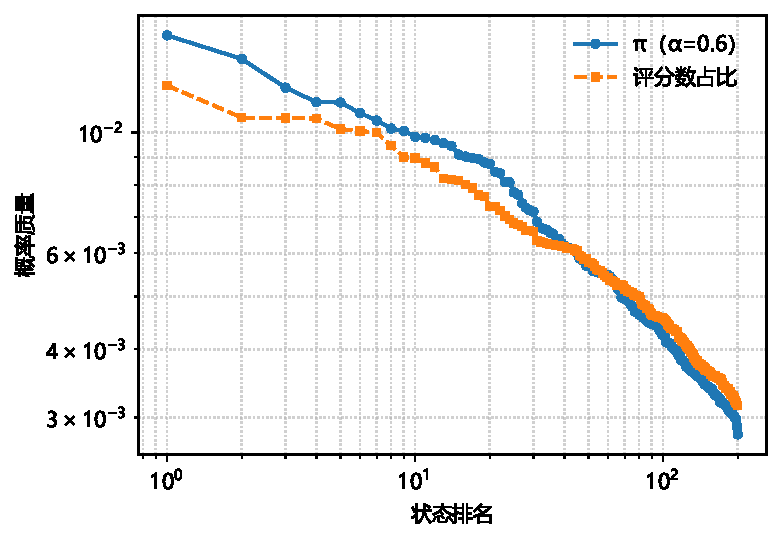
\includegraphics[width=0.56\textwidth]{fig/longtail.pdf}
\caption{$\pi$ 与纯评分数占比的长尾对比（双对数坐标）。}
\label{fig:longtail}
\end{figure}

\subsection{问题 4：历史分布分析与未来分布预测}

\subsubsection{时间切片与逐片重估}

按评分时间戳的四分位切为四个等规模时间片（表 \ref{tab:slices}），每片约 $11{,}957$ 条评分；用户数由 $270$ 增至 $359$，数据规模随时间扩张。对每片按同一规则重建图与 $P^{(t)}$，并在固定 $\alpha^*$ 下求 $\pi_t$。熵由 $5.214$ 缓慢升至 $5.235$，分布随时间略微变平，新增评分带来的多样性是主因。

\subsubsection{全局分布预测}

预测不做“平稳分布外推”，而做一步马尔可夫推进：把第 3 片的实际分布 $f_3$ 作为当前状态分布，经 $P_{\alpha^*}$ 推进一期，
\begin{equation}
\hat p_4=f_3\,P_{\alpha^*},\qquad \hat p_4\leftarrow \hat p_4/\|\hat p_4\|_1 .
\label{eq:forecast}
\end{equation}
这对应马尔可夫预测中\textbf{“分布 $\to$ 转移 $\to$ 新分布”}的语义；$\pi_t$ 仅为平稳分布，若直接作为预测值，等同于把“极限”视为“下一期”，属概念错位（附录保留该对照实验，$KL$ 由 $0.0451$ 恶化至 $0.0613$）。

评价指标为
\begin{equation}
D_{\mathrm{KL}}(f_4\|\hat p_4)=\sum_{i} f_4(i)\log\frac{f_4(i)}{\hat p_4(i)},
\label{eq:kl}
\end{equation}
以及全局 Top-10 命中率与 Spearman 秩相关 $\rho$。结果见表 \ref{tab:pred} 与图 \ref{fig:timeslice}。

\begin{table}[H]
\centering
\caption{第 4 时间片全局分布预测对比（$\alpha^*=0.6$）}
\label{tab:pred}
\small
\begin{tabular}{lccc}
\toprule
模型 & KL 散度 & Top-10 命中率 & Spearman $\rho$ \\
\midrule
\textbf{本模型：}$\hat p_4=f_3P_{\alpha^*}$ & \textbf{0.0451} & 0.30 & \textbf{0.781} \\
基线 1：纯频次 $f_{1:3}$ & 0.0585 & \textbf{0.60} & 0.642 \\
基线 2：无重启链 $\alpha=1$ 的极限分布 & 0.1353 & 0.10 & 0.443 \\
基线 3：ItemCF 单步得分 & 0.1003 & 0.10 & 0.326 \\
\midrule
对照：$\alpha=0.85$ 的一步预测 & 0.0601 & 0.20 & 0.749 \\
对照：$\pi_1,\pi_2,\pi_3$ 的均值 & 0.0613 & 0.20 & 0.679 \\
\bottomrule
\end{tabular}
\end{table}

三点结论：

\begin{enumerate}[label=(\arabic*),leftmargin=2.2em]
\item \textbf{整体分布更准}：KL 散度 $0.0451$，比纯频次 $0.0585$ 低 $23\%$，比无重启链与 ItemCF 低一个量级；秩相关 $0.781$ 也最高。说明把“共同评分结构”纳入转移后，预测的整体形状更贴近真实。
\item \textbf{Top-10 不占优}：命中率 $0.30$ 明显低于纯频次的 $0.60$。原因是本模型把质量向“与当前热门相似但非最热”的中部节点推移，整体分布更准但头部排序被打散；而纯频次在“猜最热”这一件事上有天然优势，这在评分人数高度集中的数据集上是结构性事实，不是模型缺陷。
\item \textbf{重启项是正收益}：同一预测框架下，$\alpha=0.85$ 的 KL 为 $0.0601$、命中率 $0.20$，均不如 $\alpha^*=0.6$；无重启链（$\alpha=1$）最差（KL $0.1353$）。重启项既保证平稳分布唯一，也直接改善预测质量。
\end{enumerate}

\begin{figure}[H]
\centering
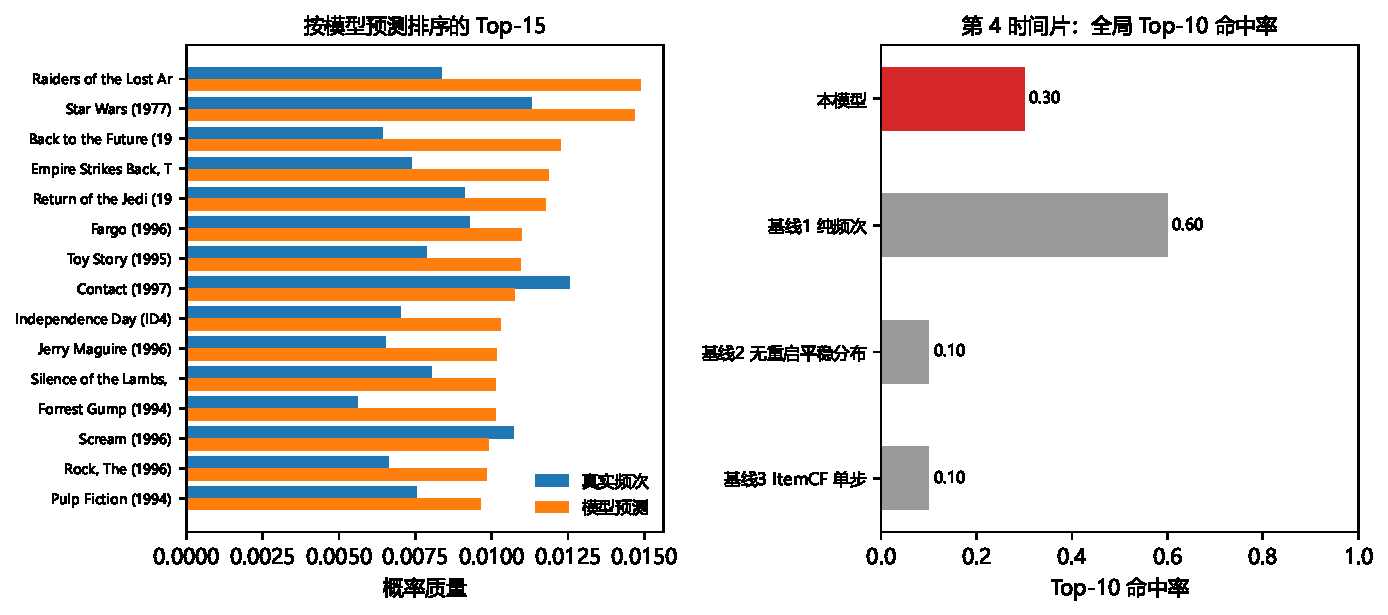
\includegraphics[width=0.96\textwidth]{fig/timeslice.pdf}
\caption{左：按模型预测排序的 Top-15，蓝色为第 4 片真实频次，橙色为模型预测；右：全局 Top-10 命中率对比。}
\label{fig:timeslice}
\end{figure}

\subsubsection{用户级个性化预测}

全局分布回答“整体热度如何变化”，个性化预测回答“为单个用户推荐什么”。评估协议严格区分验证集与测试集，避免以测试集调参：

\begin{itemize}[leftmargin=1.6em]
\item \textbf{验证集}：用第 1--2 片估计 $P$，预测第 3 片，$\alpha$ 在 $0.30$--$0.95$ 间取 $9$ 个值扫描，以 NDCG@10 为主指标选出 $\alpha^*=0.6$（$109$ 位合格用户）；
\item \textbf{测试集}：用第 1--3 片估计 $P$，预测第 4 片（$104$ 位合格用户，历史评分 $\ge5$ 条且第 4 片至少有 $1$ 条 $\ge4$ 分评分）；
\item 合格用户的种子向量由历史评分构造，边权 $w=r-2$（下限 $0.1$），按式 \eqref{eq:vu} 正则化；
\item 推荐时屏蔽用户已评过分的物品，相关物品定义为第 4 片中评分 $\ge4$ 的物品。
\end{itemize}

\begin{table}[H]
\centering
\caption{用户级个性化预测（第 4 时间片，104 位用户）}
\label{tab:user}
\small
\begin{tabular}{lccccc}
\toprule
方法 & hit@10 & P@10 & R@10 & NDCG@10 & 覆盖率 \\
\midrule
\textbf{本模型 PPR（$\alpha^*=0.6$）} & 0.577 & 0.160 & \textbf{0.195} & \textbf{0.211} & \textbf{0.635} \\
纯热门排序 & \textbf{0.577} & 0.150 & 0.184 & 0.200 & 0.365 \\
ItemCF & 0.500 & \textbf{0.164} & 0.136 & 0.200 & 0.640 \\
无重启随机游走 & 0.452 & 0.155 & 0.123 & 0.178 & 0.470 \\
\bottomrule
\end{tabular}
\end{table}

解读如下：

\begin{enumerate}[label=(\arabic*),leftmargin=2.2em]
\item \textbf{NDCG 与召回最优}：NDCG@10 达 $0.211$，高于纯热门的 $0.200$ 与 ItemCF 的 $0.200$；召回 $0.195$ 也是最高。说明排序把“用户真正会打高分”的物品放得更靠前，而不只是命中数量。
\item \textbf{覆盖率显著提升}：$0.635$ 对纯热门的 $0.365$ 提高 $74\%$。热门基线给所有人推同一批电影，覆盖率天然低；重启链让不同种子走到不同邻域，长尾物品获得曝光，这正是个性化的实际价值。
\item \textbf{命中率与热门持平}：$0.577$ 与纯热门相同。这条“没有赢”的结果需要如实保留：在只有 $200$ 部头部电影构成的封闭候选集里，热门本身就极强，任何个性化方法都难在 hit@10 上大幅超越。若把候选集扩到全库，热门基线的相对优势会下降，但本文未做该实验，不作外推。
\item \textbf{重启项的作用}：无重启随机游走（$\alpha=1$）四项指标全部垫底（hit@10 $0.452$、NDCG $0.178$），因为种子信息在自由游走中被图结构稀释，且收敛慢（$289$ 次迭代），与定理 \ref{thm:unique} 的结论一致。
\end{enumerate}

图 \ref{fig:user} 左侧为四种方法对比，右侧为 $\alpha$ 的探索--利用权衡：$\alpha$ 由 $0.30$ 增至 $0.95$ 时，命中率由 $0.606$ 降至 $0.500$；覆盖率则先由 $0.610$ 升至 $0.640$（$\alpha\approx0.55$），随后回落至 $0.480$，中间存在明显最优点。验证集选出的 $\alpha^*=0.6$ 位于“准确率仍高、覆盖率仍好”的折中区间，而非极端取值。

\begin{figure}[H]
\centering
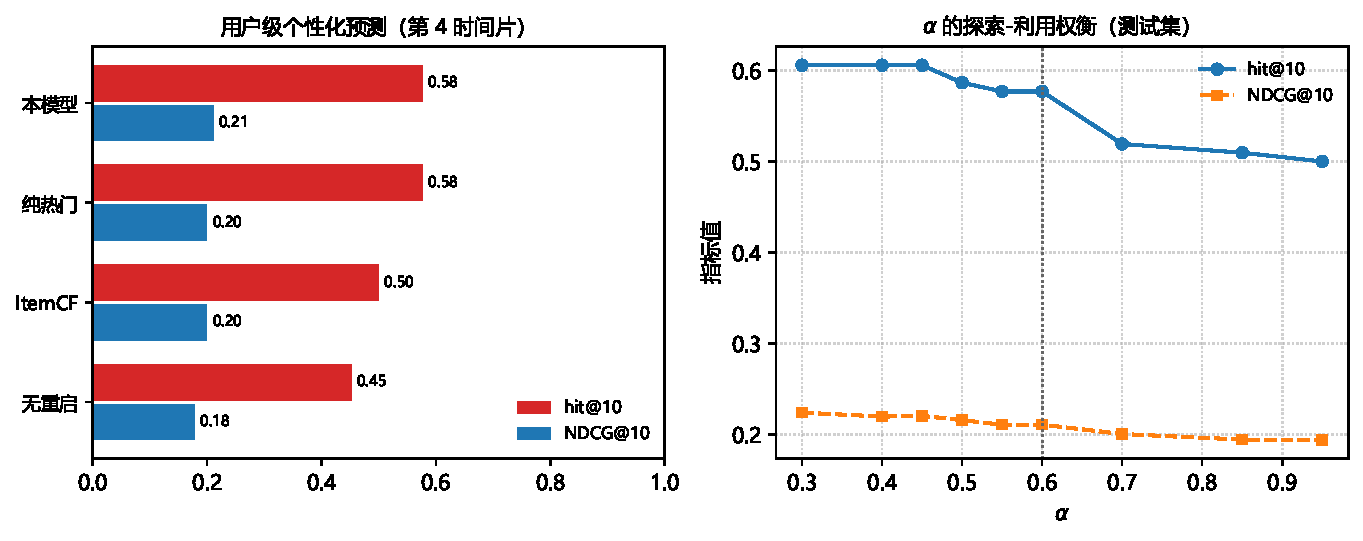
\includegraphics[width=0.96\textwidth]{fig/user_level.pdf}
\caption{左：用户级个性化预测的四方法对比；右：测试集上 $\alpha$ 的探索--利用权衡（虚线为验证集选出的 $\alpha^*=0.6$）。}
\label{fig:user}
\end{figure}

% ============================ 4 结论 ============================
\section{结论}

本文以 MovieLens 100K 为数据，将电影共现关系建成加权图，并在图上构造带重启项的随机游走马尔可夫链，从而对四个问题统一求解。主要结论如下（数值取自 \texttt{数据/results.json}，与正文表格同源）：

\begin{enumerate}[label=(\arabic*),leftmargin=2.2em]
\item \textbf{状态空间}：取评分数前 $200$ 部电影为有限状态空间，全网连通、无孤立节点；但按时间切片后第 1、2 片出现 $5$ 个连通分量与 $4$ 个悬挂节点，原链在这些片上是可约的，说明“可约性”是数据分段后的真实风险，而非人为假设。
\item \textbf{转移矩阵}：以评分向量余弦相似度定义边权、Top-20 截断并对称化，行归一化得到 $P$，非零率仅 $15.2\%$，单次乘法复杂度 $O(|E|)$，为幂迭代提供了工程可行性。
\item \textbf{极限分布}：$P_{\alpha}$ 的元素有正下界 $(1-\alpha)v_j$，故不可约非周期，平稳分布存在唯一且等于极限分布，$\alpha=0.6$ 时 $40$ 次迭代收敛，残差 $9.19\times10^{-13}$，与直接解相差 $1.13\times10^{-12}$。必须强调，这个 $\pi$ 是 $P_{\alpha}$ 的平稳分布，不是 $P$ 的；$\alpha=1$ 时二者重合且个性化项消失，数值上更换种子结果不变。
\item \textbf{历史与预测}：四个时间片的 $\pi_t$ 熵由 $5.214$ 升到 $5.235$，分布缓慢变平；用 $\hat p_4=f_3P_{\alpha^*}$ 做一步预测，KL $0.0451$、Spearman $0.781$，均为四组方法最优；用户级个性化预测 NDCG@10 $0.211$ 最优、覆盖率 $0.635$（纯热门 $0.365$），但 hit@10 与纯热门持平（$0.577$）。这说明本模型的优势在于“排序质量与覆盖面”，而不是“猜最热”。
\end{enumerate}

本文的局限有三点：候选集限定为评分数前 200 部电影，结论不宜外推至全库；余弦相似度未作用户均值中心化，对评分尺度差异不敏感；时间片仅四段且预测仅推进一步，多步误差累积尚未评估。后续可从三方面推进：将状态空间扩至全库并分层抽样、为边权引入时间衰减、以多步滚动预测检验稳定性。

% ============================ 参考文献 ============================
\newpage
\begin{thebibliography}{99}
\small
\setlength{\itemsep}{0.2em}
\addcontentsline{toc}{section}{参考文献}

\bibitem{norris} Norris J R. Markov Chains[M]. Cambridge: Cambridge University Press, 1998.

\bibitem{pf} Seneta E. Non-negative Matrices and Markov Chains[M]. 2nd ed. New York: Springer, 2006.

\bibitem{levin} Levin D A, Perron M. Markov Chains and Mixing Times[M]. 2nd ed. Providence: American Mathematical Society, 2017.

\bibitem{page} Page L, Brin S, Motwani R, Winograd T. The PageRank citation ranking: bringing order to the web[R]. Stanford: Stanford InfoLab, 1999.

\bibitem{haveliwala} Haveliwala T H. Topic-sensitive PageRank[C]//Proceedings of the 11th International Conference on World Wide Web. Honolulu, 2002: 517--526.

\bibitem{jeh} Jeh G, Widom J. SimRank: a measure of structural-context similarity[C]//Proceedings of the 8th ACM SIGKDD International Conference on Knowledge Discovery and Data Mining. Edmonton, 2002: 538--543.

\bibitem{fouss} Fouss F, Pirotte A, Renders J M, Saerens M. Random-walk computation of similarities between nodes of a graph with application to collaborative recommendation[J]. IEEE Transactions on Knowledge and Data Engineering, 2007, 19(3): 355--369.

\bibitem{movielens} Harper F M, Konstan J A. The MovieLens datasets: history and context[J]. ACM Transactions on Interactive Intelligent Systems, 2015, 5(4): 1--19.

\end{thebibliography}

% ============================ 附录 ============================
\newpage
\appendix
\section{复现说明与交付物清单}

\subsection{文件结构}

\begin{verbatim}
https://github.com/ttbr5145/markov-rwr-movielens/
  代码/preprocess.py     构图与导出（graph.json、model.npz）
  代码/compute.py        幂迭代、交叉验证、时间片、基线、全部图表
  代码/build_web.py      把 JSON 内联进单文件网页
  数据/ml-100k/          MovieLens 原始数据（u.data、u.item）
  数据/graph.json        节点/边/布局坐标
  数据/results.json      论文全部数值的唯一来源
  网页/index.html        离线可运行的单文件交互原型（约 103 KB）
  论文/paper_team.tex    团队版源码（六人）
  论文/paper_solo.tex    个人版源码（吴桐）
  论文/fig/*.pdf         7 张插图
\end{verbatim}

\subsection{运行命令}

\begin{verbatim}
python 代码/preprocess.py     # 生成图与 model.npz
python 代码/compute.py        # 生成 results.json 与 fig/*.pdf
python 代码/build_web.py      # 生成 网页\index.html
xelatex 论文/paper_solo.tex   # 个人版（两遍）
xelatex 论文/paper_team.tex   # 团队版（两遍）
\end{verbatim}

\noindent 注：数据目录 \texttt{ml-100k} 为 GroupLens 发布的 MovieLens 100K 原始数据，因体量与版权未纳入仓库；复现时需先从 GroupLens 下载 \texttt{ml-100k.zip} 解压到该目录，仓库内其余文件已齐备。

\subsection{一致性自检}

\begin{itemize}[leftmargin=1.6em]
\item 幂迭代解与直接解 $L_1$ 差 $1.13\times10^{-12}$，直接解残差 $7.25\times10^{-16}$；
\item 网页展示的 $\pi$、Top-10、四个预测指标全部来自 \texttt{results.json}，与论文表格同源；
\item 网页的 $P$ 由 \texttt{graph.json} 的边权在前端重新行归一化，与 Python 端构造一致；行和校验失败数为 $0$。
\end{itemize}

\subsection{网页交互与论文结论的对应}

\begin{table}[H]
\centering
\small
\begin{tabular}{p{0.42\textwidth}p{0.50\textwidth}}
\toprule
交互 & 对应结论 \\
\midrule
点击节点设种子，粒子从种子出发 & $P_{\alpha}$ 的幂次演化，定理 \ref{thm:unique} 的收敛性 \\
$\alpha$ 滑杆实时重排 Top-10 & 表 \ref{tab:alpha}：$\alpha$ 控制热门/冷门与混合速度 \\
关闭重启项 & $\alpha=1\Rightarrow P_{\alpha}=P$ 且与 $v$ 无关，个性化失效 \\
时间片滑杆 & 表 \ref{tab:slices}：逐片 $\pi_t$ 与推荐漂移 \\
$P_{\alpha}$ 热图悬停 & 式 \eqref{eq:Palpha-ij} 的底噪与对角块结构 \\
预测对比表 & 表 \ref{tab:pred} 的四个指标 \\
\bottomrule
\end{tabular}
\end{table}

\end{document}
